\documentclass[final,pdftex]{../../template/epsilonj}

\RequirePackage{graphicx}
\RequirePackage[colorlinks,citecolor=blue,urlcolor=blue]{hyperref}

\addbibresource{../../template/epsilon.bib}

\begin{document}

% \microtypesetup{protrusion=false, expansion=false}
\begin{frontmatter}
\title{Новости CrossValidated: выпуск 1}
\runtitle{Новости CrossValidated: выпуск 1}

\begin{aug}
\author{\imya{Андрей} \fam{Костырка}}%


\runauthor{Костырка А. В.}

\address{НИУ ВШЭ, Москва.}
\end{aug}

\begin{abstract}
	В этом разделе представлены компиляции ответов на наиболее интересные вопросы, задававшиеся на сайте \ENGs{StackExchange} в разделе «Статистика» (stats). К каждому вопросу приводятся один или несколько ответов, получивших наибольшее количество пользовательских голосов. Мнение авторов ответов может не совпадать со мнением редакции.
\end{abstract}

\begin{keyword}
	\kwd{статистика}
	\kwd{вопросы}
	\kwd{ответы}
	\kwd{интернет}
\end{keyword}

\end{frontmatter}

% \microtypesetup{protrusion=true, expansion=true}

\section{Что такое over-fitting?}

\textbf{Вопрос.} Где в реальной жизни чаще всего возникает проблема \textit{переподгонки} (переобучения "--- не в смысле «обучения заново», а в смысле «чрезмерного обучения»)? Чем плоха чрезмерно точная подгонка модели под данные?

Исходный вопрос: \url{http://stats.stackexchange.com/q/128616}.

\subsection{Подгонка под особенности шума}

Зачастую набор данных является слишком простым, а модель "--- слишком «продвинутой», из-за чего оценивание даёт ложные либо нестабильные результаты оценивания. Дополнительные параметры сложных моделей иногда оцениваются по особенностям случайного шума, который совершенно не связан с самой структурой данных, но может образовывать статистические артефакты в единичной реализации. 

\subsection{Модель плохо работает за пределами выборки}

Несмотря на свою примитивность, линейные модели довольно неплохо дают общее представление об устройстве данных. Если же точки располагаются вдоль воображаемого нелинейного облака точек, то тогда специфические математические функции (экспонента, логарифм, полином $k$-й степени, синус и~проч.) принимают значения, более близкие к значениям набора данных, однако за границами определённого диапазона их поведение теряет адекватность интерпретации.

Рассмотрим динамику населения США в XX~веке (рис.~\ref{fig:usa}). Линейная модель довольно хорошо описывает данные. Полином шестой степени более точно проходит через имеющиеся точки, однако даёт прогноз, согласно которому к 2050~году всё население США загадочным образом исчезнет. Подобное экстраполирование абсурдно, поэтому этот пример "--- классический случай переподгонки.

\begin{figure}[htbp]
	\centering
	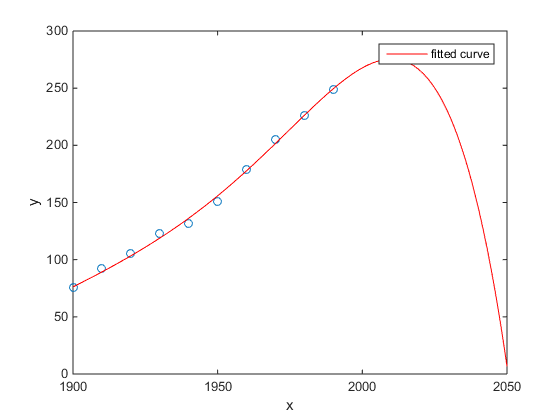
\includegraphics[width=9cm]{overfit.png}
	\caption{Over-fitting динамики населения США} \label{fig:usa}
\end{figure}

\subsection{Система Птолемея}

Птолемей полагал, что Земля находится в центре Вселенной, и вывел громоздкую систему вложенных сферических орбит, хорошо объяснявшую движение небесных тел. Однако реальные измерения систематически отличались от прогнозов, реализуемых в рамках системы Птолемея, поэтому асторономам"=геоцентристам приходилось придумывать всё больше дополнительных сфер, пока, наконец, модель не стала настолько запутанной, что начала вызывать подозрения в истинности предпосылок, на которых основывалась.

\subsection{Не бывает переподгонки процесса, порождающего данные}

Сам по себе DGP (\ENGs{data-generating process}) переподогнать невозможно. Мы не знаем истинного DGP, но лишь пытаемся его моделировать. Так как DGP один, то и истинная модель может быть только одна, а все остальные содержат ошибки спецификации того или иного уровня. В социальных науках большинство моделей принципиально неполные или неправильно специфицированные, поэтому усложнённые модели захватывают особенности доступного набора данных, а не процесса, стоящего за ними.

\subsection{Боязнь пропущенных переменных}

Многие эконометристы полагают, что пропущенные переменные "--- это опаснейшая проблема, куда более острая, чем избыточные переменные. Чтобы выбрать из двух зол наименьшее, некоторые из этих эконометристов добавляют в модель степени регрессоров, а также всевозможные пересечения (кросс"=произведения) и иррелевантные переменные. В самом общем случае добавление в уравнение множественной регрессии всех доступных в наборе переменных, которые могут потенциально обладать объясняющей силой, является переподгонкой: исследователь наблюдает не генеральную совокупность, а только выборку, поэтому он не может знать, какая из всех возможных спецификаций является верной.

Как водится, есть две новости: хорошая и плохая. Хорошая новость: включение лишних переменных не приводит к смещению оценок коэффициентов при значимых. Плохая новость: точность оценивания релевантных коэффициентов падает, ошибка регрессии растёт, доверительный интервал прогноза расширяется.

\subsection{Мнение редактора}

Два критерия качества модели "--- \ENGs{goodness of fit} (подгонка) и \ENGs{goodness of forecast} (прогноз) "--- зачастую бывают недостижимы одновременно. Представьте себе отличную базу панельных данных с одним миллионом индивидов, каждый из которых наблюдается в течение пяти-десяти лет (такие базы, например, имеются в распоряжении у французских статистических органов, а также у сотрудников Национальной школы статистики). Представим, что мы строим зарплатное уравнение в зависимости от стажа, пола, образования, возраста с квадратом и других стандартных факторов. Каждый индивид обладает своим индивидуальным эффектом, который легче всего измерить при помощи дамми"=переменной для этого самого индивида. Предположим, у нас есть 8\,000\,000 наблюдений и 1\,000\,005 оцениваемых при помощи МНК коэффициентов (стаж, пол, возраст с квадратом, образование и миллион дамми). Оценённая модель будет обладать фантастически высоким показателем $R^2$ и отлично объяснять устройство данных; почти все коэффициенты при этом будут значимы! Однако представим, что в выборку попадает новый индивид "--- одна новая точка. Оценки индивидуального эффекта для него у нас попросту нет. Каким будет прогноз его заработной платы? Как в старом анекдоте: «Насчёт СССР мы не знаем, но на китайско"=финской границе всё будет спокойно!»

Ещё более гипертрофированный пример: есть срез из 1\,000\,000~индивидов в один момент времени, и для каждого индивида в уравнение регрессии добавляется его дамми. Такая модель объяснит 100\,\% вариабельности переменной дохода, однако будет неспособна предсказать доход новых респондентов.

\subsection{Вопрос читателям}

Придумайте для какого"=либо набора данных модель, которая обладает очень хорошей прогнозной силой (довольно точно предсказывает значения для точек как внутри диапазона значений "--- где модель оценивалась, "--- так и за его пределами "--- где необходимо угадать свойства объекта, не участвовавшего в обучении), однако скверной объясняющей способностью.

\section{Следует ли из причинно"=следственной связи корреляция?}

\textbf{Вопрос.} Многие студенты второго курса бывали биты за то, что утверждали, будто бы из корреляции следует каузальность, т.\,е. «они коррелируют, следовательно, одно является причиной другого». Любой зарубежный студент"=отличник на устном экзамене повторяет мантру «\ENGs{correlation does not imply causation}». Предположение о независимости случайных величин всегда сильнее предположения об их некоррелированности. Однако верно ли обратное? Обязательно ли из причинно"=следственной связи следует корреляция?

Исходный вопрос: \url{http://stats.stackexchange.com/q/26300}.

\subsection{Линейная корреляция}

Если понимать под корреляцией общую корреляцию Пирсона, рассчитываемую по формуле
\[
\Corr(X,Y) = \frac{\Cov(X,Y)}{\sqrt{\Var(X) \Var(Y)}},
\]
то причинно"=следственная связь двух переменных не всегда приводит к возникновению линейной корреляции. Достаточно рассмотреть такой набор данных, как точки, лежащие на прямой $y = x^2$ в любом симметричном относительно начала координат диапазоне. В данном случае зависимость будет функциональной, однако коэффициент корреляции Пирсона будет равен нулю. Во многих справочниках присутствует изображение (рис.~\ref{fig:corr}\footnote{Исходный примет взят с \url{en.wikipedia.org/wiki/File:Correlation_examples2.svg}.}), на котором показано, что у многих наборов данных две переменные явно связаны некоторой зависимостью, однако линейная корреляция равна нулю.

\begin{figure}[htbp]
	\centering
	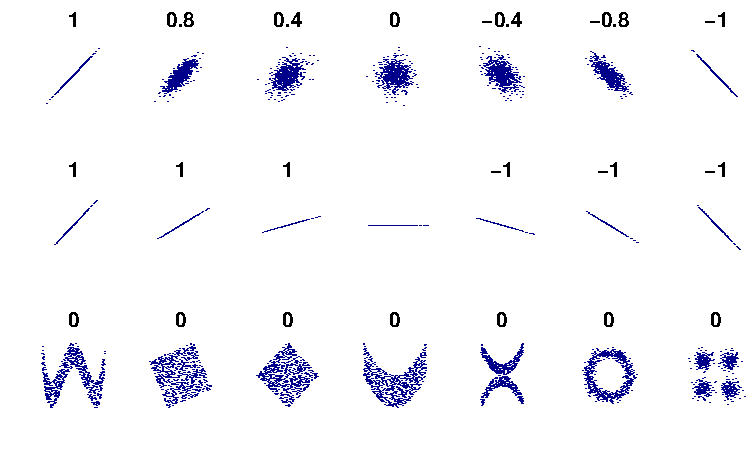
\includegraphics[width=9cm]{corr-image.pdf}
	\caption{Коэффициенты корреляции в различных наборах данных} \label{fig:corr}
\end{figure}

Более подходящий термин для данного вопроса "--- это «взаимная информация». Справедливо утверждение о том, что причинно"=следственная связь влечёт высокую \textit{взаимную информацию}. Последняя имеет более сложное определение, чем корреляция, и измеряет уменьшение неопределённости относительно одной случайной величины при поступлении информации о другой случайной величине.

Следует помнить, что если некоторая причина влечёт некоторое следствие и при этом эта причина идеально коррелирует с другой причиной, вызывающей противоположный результат, то корреляция этих двух причин и следствия равна нулю. Однако в действительности такой идеальной линейной зависивости между двумя причинами со строго противоположными эффектами не существует, поэтому не следует полагать, что такие причины существуют вообще. Пример: единороги вызывают некоторое явление, гномы оказывают точно такое же противодействие, а посему итоговый эффект равен нулю.

\subsection{Теоретический контрпример}

Рассмотрим две случайные величины: $X\sim\calN(0;1)$, $Y=X^2$. По определению $Y\sim \chi^2_1$. Трудно придумать более сильную причинно"=следственную связь: $X$ полностью определяет $Y$. Мы видим, что $\E(X)=0$, $\E(Y)=1$. Вычислим значение коэффициента ковариации. 
\begin{multline*}
\cov(X,Y) = \E\bigl( (X - \E(X)) (Y - \E(Y)) \bigr) = \\
 = \E\bigl( (X-0)(Y-1) \bigr) = \E(XY) - \E(X) = \E(X^3) - 0 = 0
\end{multline*}
Мы воспользовались тем свойством, что нечётные центральные моменты стандартной нормальной случайной величины равны нулю. Следовательно, корреляция между ними также равна нулю.

Данное доказательство работает не только для стандартного нормального, но и вообще для любого симметричного относительно нуля распределения (равномерного от~$-a$ до~$a$, Лапласа, Стьюдента и~проч.), у которого существуют хотя бы три центральных момента. Если каждое положительное значение величины $X$ так же вероятно, как и противоположное ему, то при возведении в квадрат мы не можем сказать, связаны ли б\'{о}льшие значения квадрата случайной величины с положительными или отрицательными~$X$. 

\subsection{Эмпирический контрпример}

Если одно случайное событие является причиной другого случайного события, между ними обязана существовать некоторая взаимосвязь (односторонняя или двухсторонняя), которая может выражаться в нелинейной корреляции.

При проведении выборочных исследований домохозяйств иногда в качестве средства опроса используется телефон. При этом вероятность ответа на звонок максимальна у людей, относящихся к среднему классу в терминах дохода, и значительно ниже у очень состоятельных или, наоборот, социально незащищённых граждан. На рис.~\ref{fig:corr} видно, что параболическая зависимость переменных (нижний ряд, центральное изображение, ветви параболы могут быть направлены вверх или вниз) влечёт нулевую корреляцию. Причинно"=следственная связь вида «доход влияет на вероятность ответа по телефону» заключается в том, что на верхнем конце распределения люди предпочитают не выдавать информации о себе (в том числе и потому, что к ним зачастую обращаются по телефону с просьбой «поделиться доходами»), а на нижнем конце распределения индивиды чаще являются должниками, имеющими непогашенный долг перед банком или знакомыми, и это является причиной их более осторожного поведения.

\section{Почему вариабельность измеряют именно квадратами?}

\textbf{Вопрос.} Почему в статистике для определения меры разброса случайной величины берутся \textit{квадраты} отклонений от среднего, и почему стандартное отклонение считается как корень из мат. ожидания квадрата? Разве мат. ожидание модуля отклонений не покажет вариабельность данных? 

\begin{center}
	\begin{tabular}{cc}
		\null\quad Почему вместо \quad\null & \null\quad не используют \quad\null \\
		$\sigma = \sqrt{\E\bigl( (X - \mu_X )^2 \bigr)}$ & $\sigma = \E(|X - \mu_X|)$?
	\end{tabular}
\end{center}

Исходный вопрос: \url{http://stats.stackexchange.com/q/118}.

\subsection{Квадрат не единственная используемая функция}

В некоторых моделях используется среднее абсолютное отклонение для определения меры разброса случайных величин. Так, при диагностике моделей временных рядов качество прогноза оценивается при помощи нескольких мер: среднее относительное отклонение, среднее абсолютное отклонение, среднее квадратичное отклонение.

Кроме того, стандартное отклонение, определяемое как корень из дисперсии, не является «стандартным» в статистической науке. Точно так же и главные компоненты в одноимённом методе не являются главным инструментом учёного: это всего лишь название.

\subsection{Преимущества стандартного отклонения}

Если стандартное отклонение призвано измерить разброс данных, то стоит сперва определить этот самый разброс. Функция квадратов отклонений обладает несколькими важными свойствами:
\begin{enumerate}
	\item Функция квадрата непрерывно дифференцируема;
	\item Она является достаточной статистикой для распределения Гаусса;
	\item Она является разновидностью $L^2$-нормы, которая полезна при доказательствах сходимости;
	\item Возведение в квадрат смещает вес в сторону б\'{о}льших отклонений "--- со всеми полезными и негативными последствиями.
\end{enumerate}

Обе штрафные функции "--- квадрат и модуль "--- всегда возвращают неотрицательную величину, поэтому (за исключением вырожденного случая) сумма штрафов будет положительной.

Само по себе возведение в квадрат трудно интерпретируется, так как некоторые единицы измерения в квадрате (доллары, дни, станки) лишены физического смысла. Для возврата к оригинальным единицам считается квадратный корень из суммы.

Абсолютные отклонения (модули) назначают равные веса наблюдениям из всего диапазона значений, в то время как квадраты усиливают влияние крайних наблюдений. С алгебраической точки зрения работать намного удобнее с квадратами, в то время как модули не дают некоторых свойств (например, дисперсия равна разности мат. ожидания квадрата и квадрата мат. ожидания). 

Использование квадратов хорошо интерпретируется через статистический аналог теоремы Пифагора: $c = \sqrt{a^2 + b^2}$. Из неё также следует, что дисперсии независимых случайных величин складываются, а стандартные отклонения "--- нет. 

\subsection{Недостатки абсолютного отклонения}

Если функция модуля непрерывна всюду на $\mathbb{R}$, то её первая производная "--- нет (в нуле). Это усложняет аналитическое решение многих задач.

Если в линейной регрессии используется штрафная функция $L(e) = |e|$, то тогда полученная регрессия называется медианной, а в более общем случае ($(1-\alpha)|e|$ для $e<0$ и $\alpha|e|$ для $e\ge0$) "--- квантильной. Вычисление квантилей связано с задачами линейного программирования, которые могут становиться сложнее на порядок. При наличии $n$ точек задача минимизации суммы квадратов решается за время $O(n)$, а суммы модулей "--- за $O(n \ln n)$, так как самый общий алгоритм подразумевает поиск решения.

\subsection{Иные случаи}

Предположим, исследователю необходимо измерить очень маленькие величины сравнительно неточным прибором (например линейкой). Так как длина не может быть отрицательной, то распределение будет асимметричным, следовательно, имеет смысл оценивание параметров распределения, дающего положительные значения (бета-, гамма-, Пуассона, Фишера"--~Снедекора и~проч.). Среднеквадратичный разброс будет связан с параметрами этих распределений, однако будет хуже содержательно интерпретироваться.


\subsection{Вопрос читателям}

Чем б\'{о}льшие значения принимает штрафная функция при больших значениях аргумента, тем чувствительнее регрессия к большим выбросам, так как по сути происходит минимизация суммы с большой долей функции от максимальной компоненты. Рассмотрите два примера штрафной функции от остатков:
\begin{enumerate}
	\item $L(e) = x\cdot \ln (x+1)$;
	\item $L(e) = x\cdot \ln^2 (x+1)$;
	\item $L(e) = \sqrt{|x|}$.
\end{enumerate}
Решите нормальные уравнения для задачи $\min \sum\limits_i L(e_i)$ во всех трёх случаях для парной регрессии вида $y_i = \alpha + \beta x_i + \e_i$. 

Сгенерируйте в любой эконометрической программной среде набор данных с известными свойствами и проведите серию экспериментов Монте"=Карло, оценив в каждом случае уравнение регрессии методов наименьших штрафных функций, предложенных выше. Изучите распределение коэффициентов. Измерьте чувствительность коэффициентов к статистическим выбросам. Сравните эти оценки с оценками методов наименьших квадратов и наименьших модулей.

\section{Как преобразовывать неотрицательные данные с нулями? }

Если данные строго положительные, то в таком случае переменные иногда логарифмируют. Но что делать с неотрицательными данными, в которых присутствуют нули? Если рассматривать преобразование вида $\ln (x+c)$, то следует ли использовать $c=1$, чтобы нули обратились в нули, либо оценивать $\hat c$, либо брать очень малое положительное значение? Есть ли другие преобразования?

Исходный вопрос: \url{http://stats.stackexchange.com/q/1444}.

\section{Причины возникновения нулей}

В первую очередь необходимо изучить природу данных и понять, почему некоторые наблюдения содержат нулевые значения. Каждую из нижеслеюующих причин необходимо рассматривать в отдельности:
\begin{enumerate}
	\item Усечение или цензурирование данных (исследователь не располагает отрицательными наблюдениями, хотя они могли бы быть);
	\item Пропущенные наблюдения (если переменная содержательно должна быть положительной: цена, длительность и~проч.);
	\item Естественный ноль (доход индивида может быть равен нулю, если он безработный);
	\item Специфика чувствительности средства измерения переменной (инструмент не реагирует на количества, меньшие определённого порога).
\end{enumerate}

Предлагаемые решения:
\begin{enumerate}
	\item Использование моделей, учитывающих информацию об ограниченных значениях переменной (модель Хекмана, интервальная регрессия, модели времени жизни);
	\item Выбрасывание из модели наблюдений, содержащих пропуски, если учтены все возможные последствия этого решения;
	\item Числовое преобразование, упоминавшееся в вопросе;
	\item Использование специальных LOD-моделей (Limit of Detection), непараметрических методов, а в первую очередь "--- изучение книги \cite{nondetect05}.
\end{enumerate}

С точки зрения регрессионного анализа может быть полезно добавить дамми"=переменную для наблюдений с нулями. Последний случай является самым тяжёлым, причём в эконометрике он практически не встречается (этот вопрос более актуален для специалистов, снимающих показания с реальных датчиков, обладающих порогом чувствительности).

\subsection{Числовое преобразование}

В работе \cite{squeezer06} предлагается использовать преобразование 
\[
x' = \frac{x(N-1) + s}{N},
\]
где $N$ "--- число наблюдений, а $s$ "--- априорная вероятность для бета"=распределения (зачастую наиболее практично использовать $s=0{,}5$).

\printbibliography

\end{document}

% Процитировать:
Christopher D. Manning, Prabhakar Raghavan, Hinrich Schütze (2008). An Introduction to Information Retrieval. Cambridge University Press. ISBN 0-521-86571-9.

